This chapter examines the simulation outcomes, with a focus on key parameters influencing the results. It begins by explaining the graphs used in the analysis. Subsequently, it presents the results obtained with the default parameters and analyzes replicas of the default scenario. The sensitivity analysis follows, investigating how variations in variables such as screening frequency, screening intervals, colonoscopy costs, and FIT performance indicators impact the results. This thorough exploration provides stakeholders with insights into the factors shaping the outcomes, assisting in evidence-based decision-making and policy formulation for optimizing colorectal cancer screening and management.

\section{Results Example}
First, we will examine the graphs used in the results to better explain their significance to the analysis.

\subsection*{Treatments Bar Chart}

This bar chart illustrates the distribution of treatments by stage.

\begin{figure}[H]
    \centering
    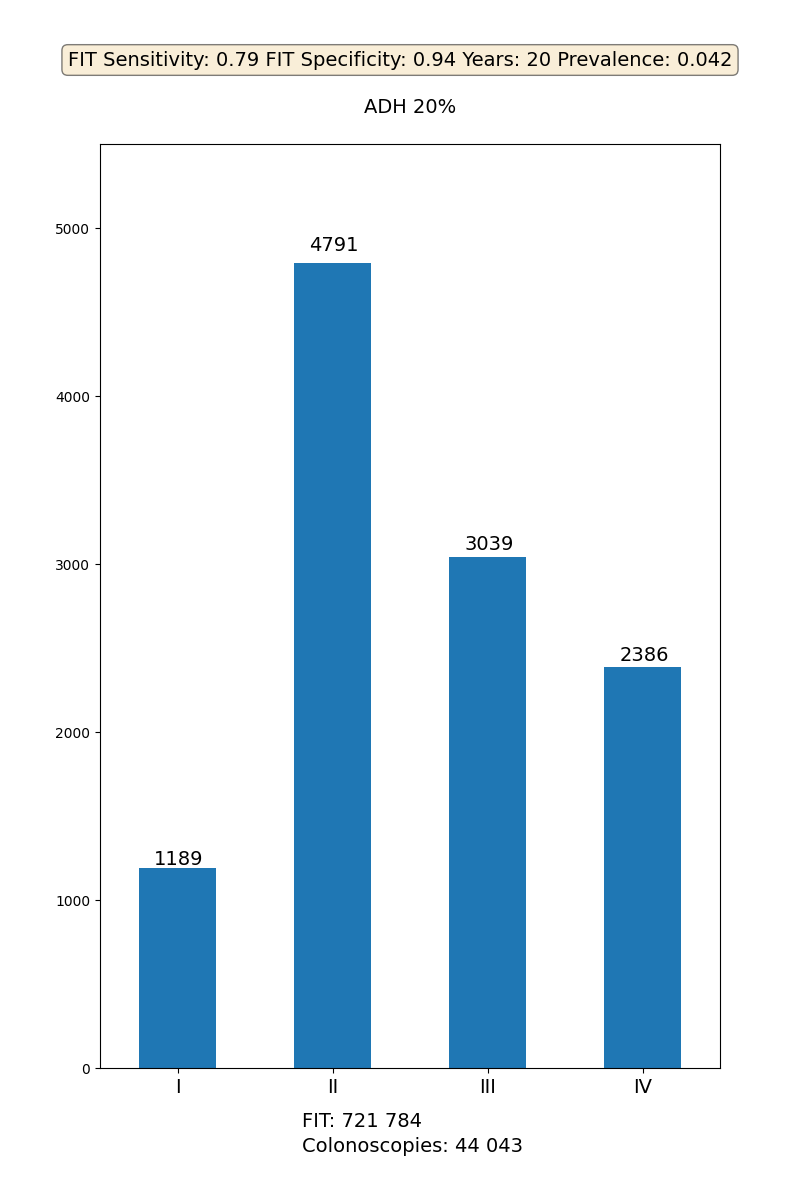
\includegraphics[scale= 0.45]{images/5.results/treatments_for_example.png}
    \caption{Example of Treatments Bar Chart}
    \label{fig:treatments_for_example}
\end{figure}

In Figure \ref{fig:treatments_for_example}, the simulation presents a single scenario, labeled "ADH 20\%" to indicate the population's adherence percentage. The yellow box displays the fixed parameters for all scenarios, while below the plot, the numbers of FIT exams and Colonoscopies performed are provided. This chart is essential for illustrating the changes in the distribution of treatment stages and the number of FIT exams and Colonoscopies performed under different scenarios.

\subsection*{Screening Efficacy Bar Chart}

This horizontal bar chart demonstrates the efficiency of the screening in detecting CRC cases during their asymptomatic period.

\begin{figure}[H]
    \centering
    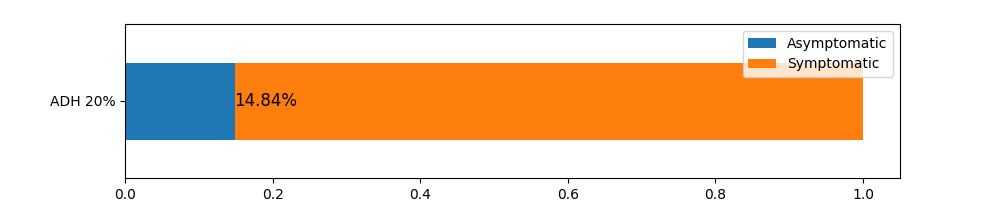
\includegraphics[scale= 0.5]{images/5.results/screening_efficacy_for_example.png}
    \caption{Example of Screening Efficacy Bar Chart}
    \label{fig:screening_efficacy_for_example}
\end{figure}

In the chart illustrated in Figure \ref{fig:screening_efficacy_for_example}, we observe the same 20\% adherence case, showing the percentage of asymptomatic treatments. This chart is valuable for comparing different scenarios and understanding how the screening strategy's effectiveness varies between them.

\begin{figure}[H]
    \centering
    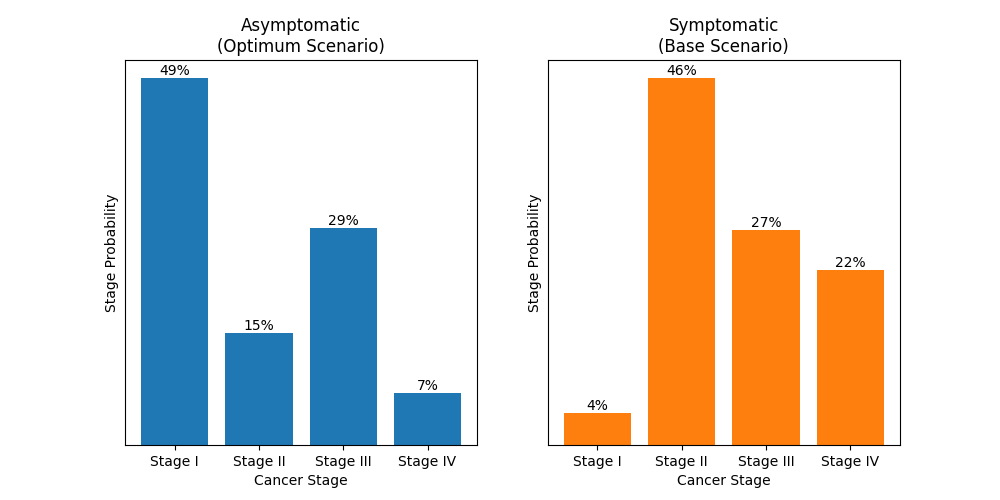
\includegraphics[width=1\textwidth]{images/4.simulation/cancer_stage_probability.png}
    \caption{Symptomatic or Asymptomatic Detection}
    \label{fig:symptomatic_vs_asymptomatic_detection_2}
\end{figure}

As depicted in Figure \ref{fig:screening_efficacy_for_example}, at 20\% adherence, approximately 15\% of all cases are treated before showing any symptoms. This implies that three out of every twenty CRC cases would align with the optimum scenario in terms of cancer stage distribution probabilities, while the remaining cases would align with the base scenario shown in Figure \ref{fig:symptomatic_vs_asymptomatic_detection_2}.

\subsection*{Costs Pie Chart}

This pie chart depicts the distribution of costs for screening and treatment procedures.

\begin{figure}[H]
    \centering
    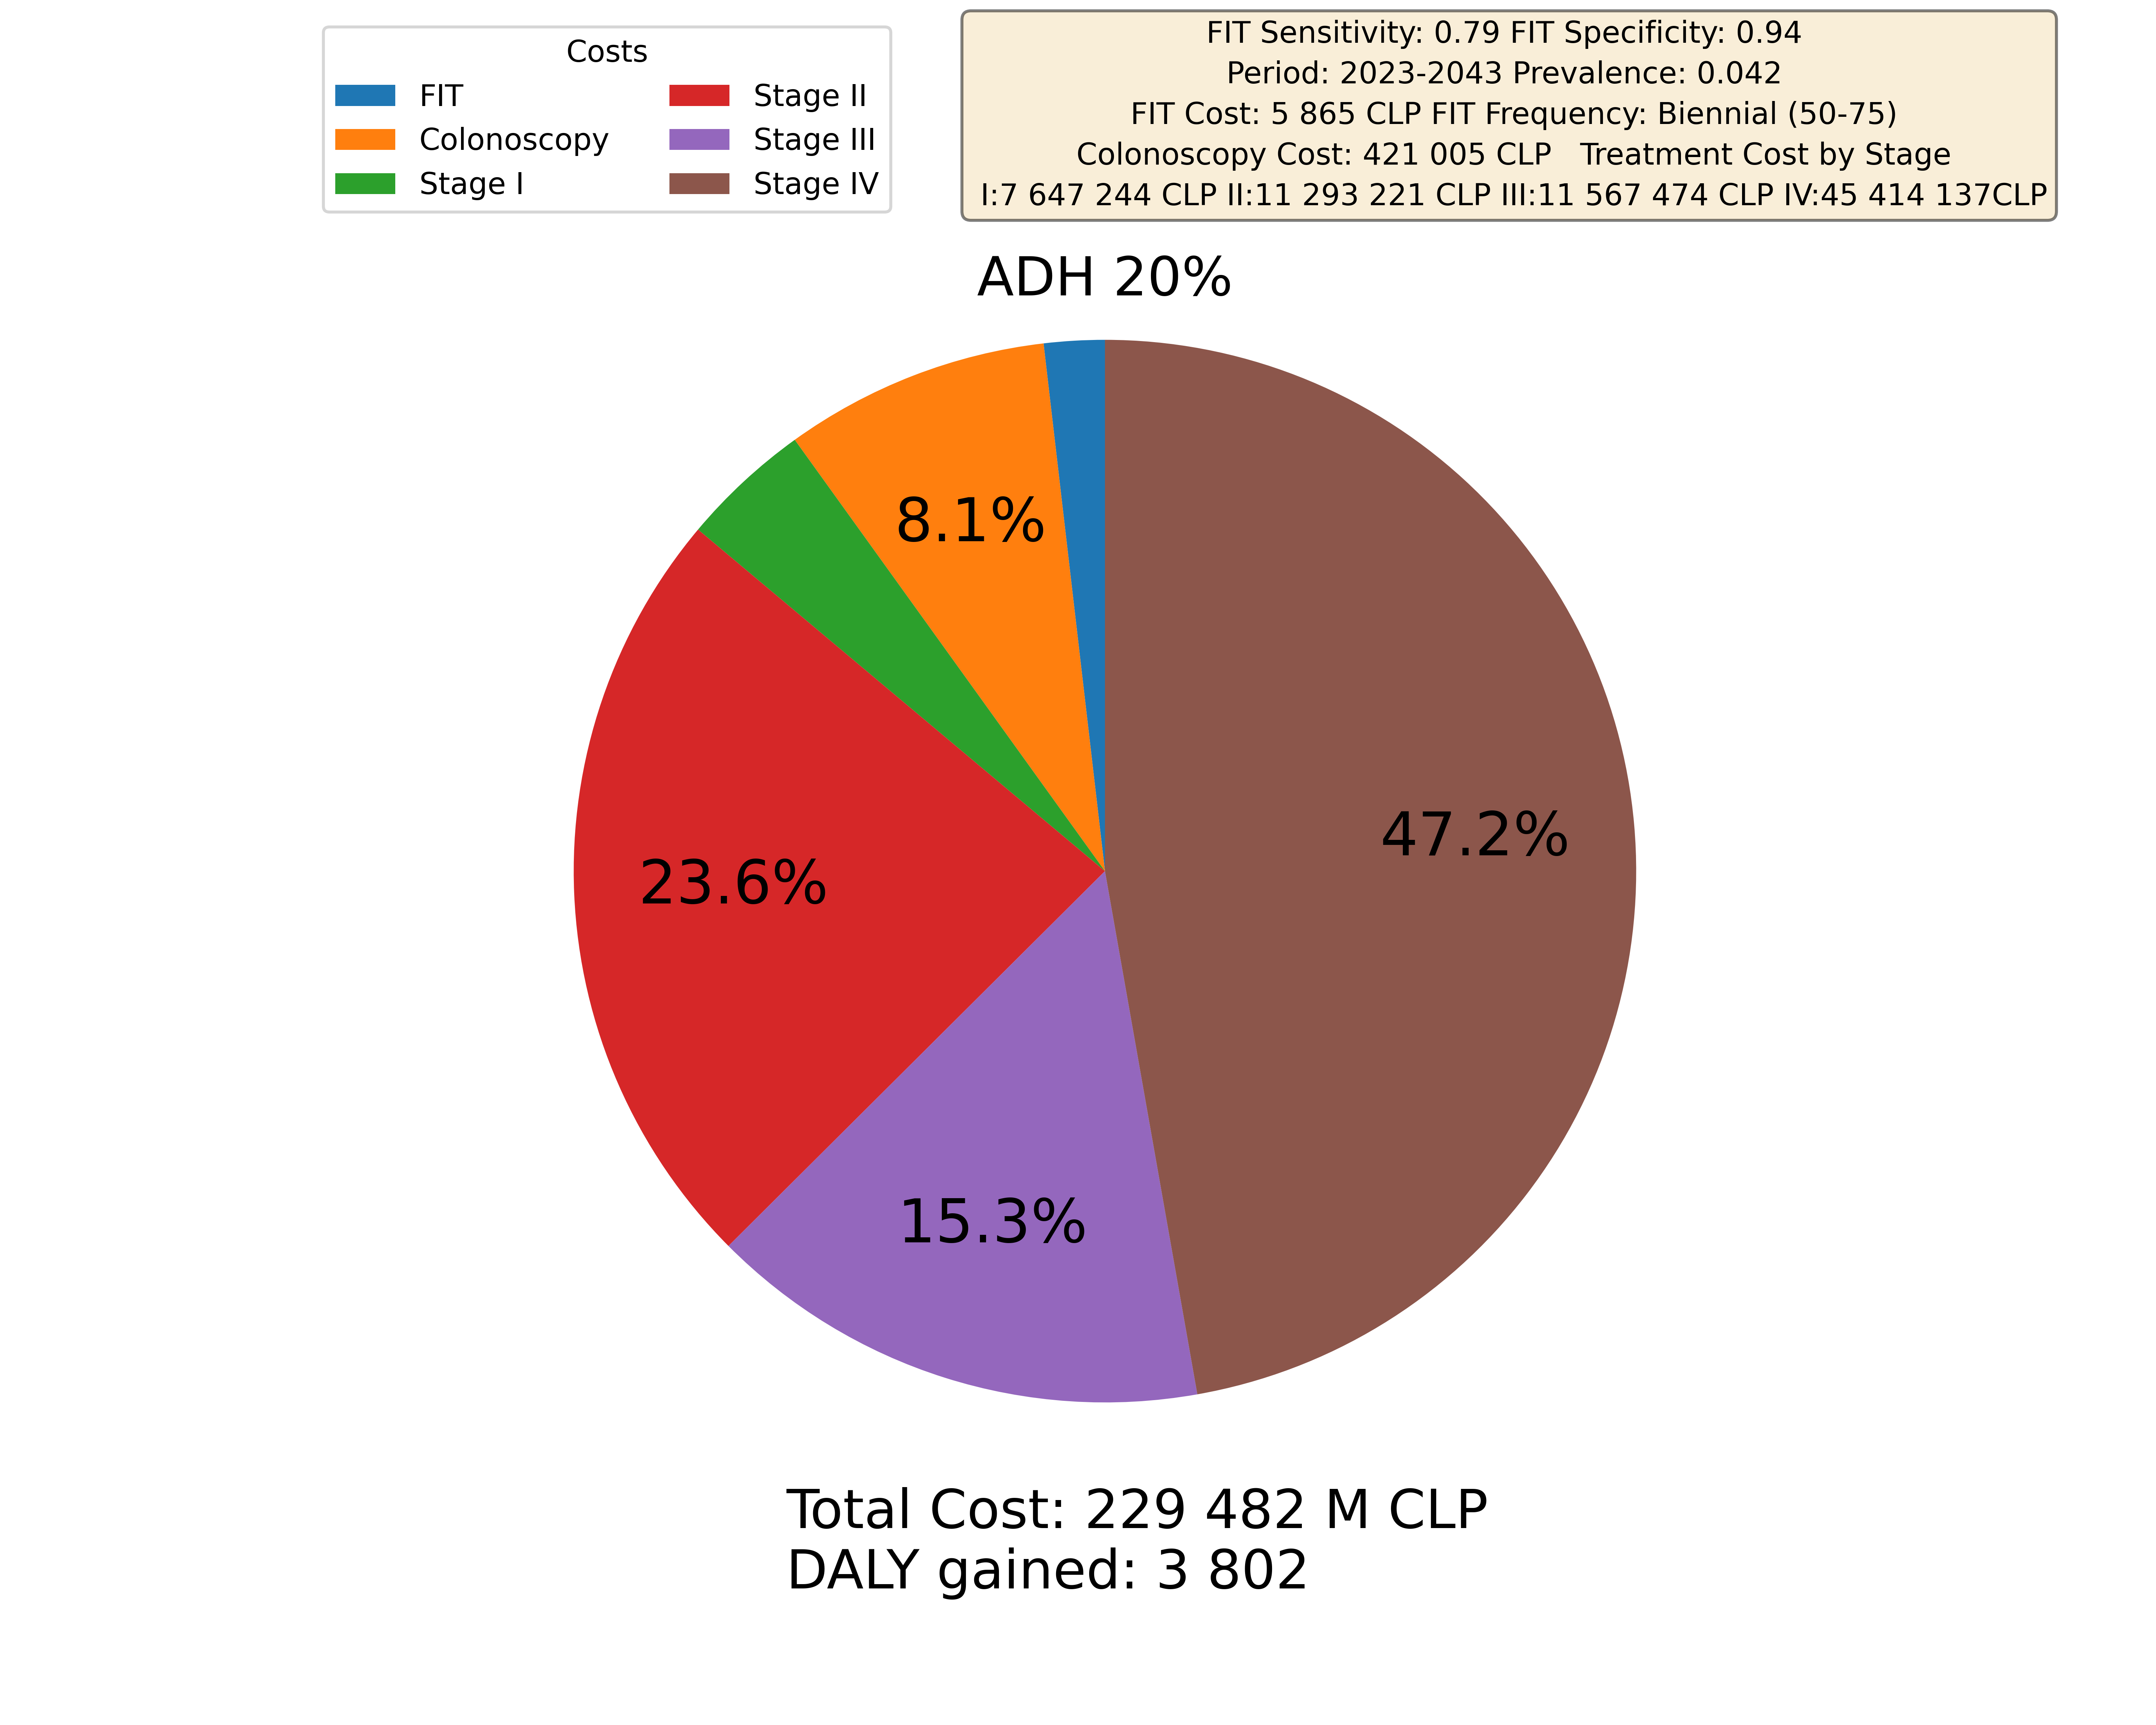
\includegraphics[scale=0.5]{images/5.results/costs_for_example.png}
    \caption{Example of Costs Pie Chart}
    \label{fig:costs_for_example}
\end{figure}

In the pie chart shown in Figure \ref{fig:costs_for_example}, we can see the six costs that constitute the CRC care process in the simulation model. The total cost and the disability adjusted life-years (DALY) gained from the screening strategy are presented below the graph. Additionally, when multiple scenarios are presented, the cost percentage difference from the base model is included. This graph serves as the primary visual support for the economic analysis of the various scenarios.

\section{Simulation Benchmarks}

The simulation results were generated using a MacBook Air with an M1 chip. The duration of each simulation varied based on the number of adherence scenarios and years simulated.

For the default simulation, which included 8 adherence scenarios, each running for 20 years, the first scenario completed in 24 seconds. In total, all 8 scenarios took 192 seconds to run. When the same 8 scenarios were simulated for 200 years, the first scenario took 257 seconds to complete, and all scenarios finished in 37 minutes.

\section{Result with the Default Parameters}

In this section, we will present the results using the default parameters. All of them where carefully described along with their sources in the \hyperref[section:simulation_parameters]{Simulation Parameters section}.

\subsection*{Effectiveness Analysis}

Assessing results independently of costs is crucial for evaluating the effectiveness of the screening strategy on CRC prognosis. This analysis allows researchers to understand the true impact of the screening approach on disease management, free from financial considerations.

\begin{figure}[H]
    \centering
    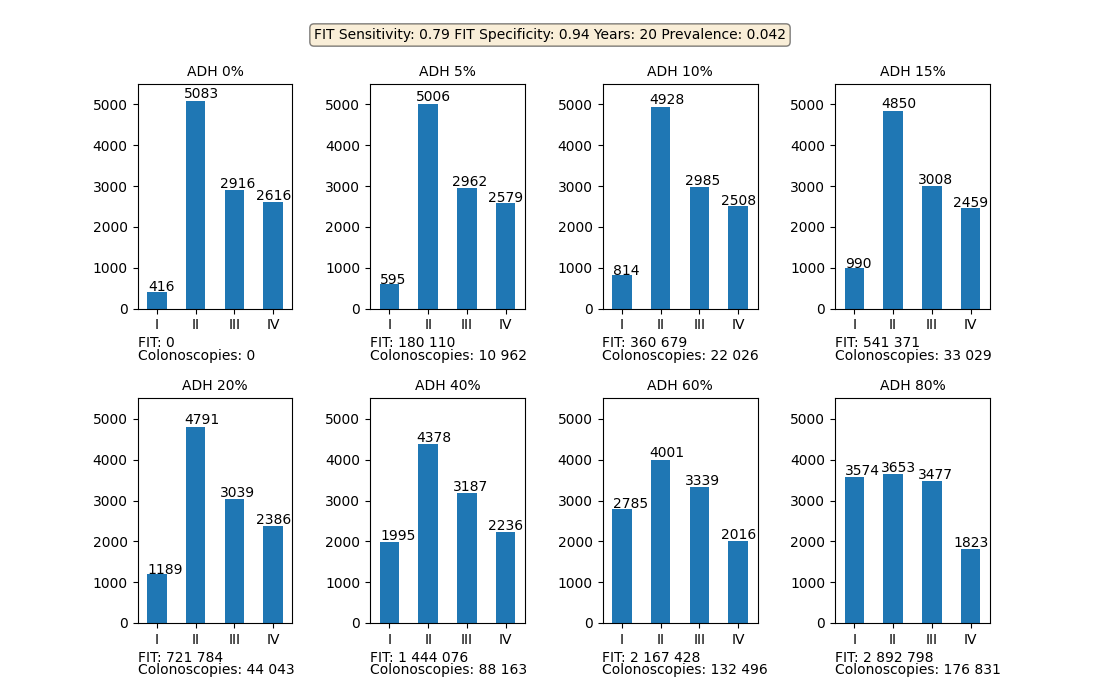
\includegraphics[width=1\textwidth]{images/5.results/treatments_by_adherence.png}
    \caption{Treatments by Adherence}
    \label{fig:treatments_by_adherence}
\end{figure}

The scenarios depicted in Figure \ref{fig:treatments_by_adherence} demonstrate a trend where higher screening adherence is associated with earlier stage treatment of cancer. At 0\% adherence, treatment primarily targets stage II, with a notable volume in stage III. As adherence increases to 5\%, 10\%, and 15\%, there is a decline in treatments for advanced stages III and IV, coupled with an increase in early-stage interventions. This trend continues at 40\%, 60\%, and peaks at 80\% adherence.

At 20\% adherence, a level that could be reasonably expected from the population in the SMPHS, there is a significant increase in resource allocation for screening exams. Approximately 36,089 FIT exams and 2,202 colonoscopies would be required annually for screening purposes alone.

\begin{figure}[H]
    \centering
    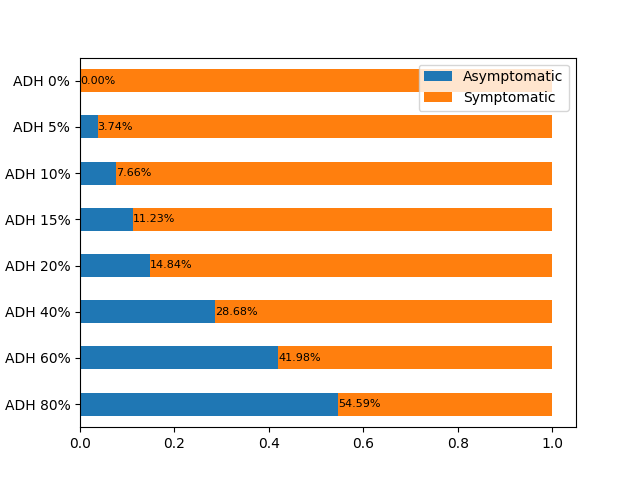
\includegraphics[width=1\textwidth]{images/5.results/screening_efficacy_by_adherence.png}
    \caption{Screening Efficacy by Adherence}
    \label{fig:screening_efficacy_by_adherence}
\end{figure}

Here, Figure \ref{fig:screening_efficacy_by_adherence} also illustrates that as adherence increases, there's a noticeable rise in asymptomatic cancer treatments, indicating earlier detection. At a population adherence of 20\%, approximately 14.8\% of all cases would be discovered during the asymptomatic period.

Graphs \ref{fig:treatments_by_adherence} and \ref{fig:screening_efficacy_by_adherence} underscore the idea that higher adherence to colorectal cancer screening leads to a shift toward earlier-stage treatment. This shift highlights the need for increased resource allocation, meaning the need for additional personnel and equipment to implement a succesful screening strategy.

\subsection*{Cost Analysis}

While the screening strategy has proven successful in improving the outcomes of earlier stage detection, it's crucial to incorporate costs into the analysis of implementation. This consideration enables decision-makers to evaluate the financial feasibility and sustainability of screening programs, ensuring the efficient allocation of resources.

\begin{figure}[H]
    \centering
    
\includegraphics[width=1\textwidth]{images/5.results/costs_by_adherence.png}
    \caption{Costs by Adherence}
    \label{fig:costs_by_adherence}
\end{figure}

The data in Figure \ref{fig:costs_by_adherence} illustrates the same eight scenarios with varying adherence levels. At 0\% adherence, most costs come from treating CRC in stages III and IV, showing a higher financial burden due to later-detected cancers. As adherence improves, costs shift towards FIT and colonoscopy procedures, with a significant reduction in treatment costs. This trend intensifies with higher adherence levels. At 80\% adherence, screening procedures account for about a quarter of total costs, highlighting a substantial investment in preventive care. Despite saving costs in treatments across all scenarios, these savings do not counterbalance the expenditure on screening procedures.

The pie charts in Figure \ref{fig:costs_by_adherence} offer a clear depiction of the cost dynamics of colorectal cancer screening and treatment. They emphasize the shift towards preventive measures with increased screening adherence, indicating potential for improved health outcomes but also an increase in overall CRC care resources.

\section{Simulation Replicas}

Due to the inherent randomness affecting each individual and the population size in each simulation instance, the outcomes should theoretically remain consistent when replicating the same scenario. To validate this, ten replicas of the default scenario were run. The outcomes of scenarios with 20\% adherence are presented in the following figures.

\begin{figure}[H]
    \centering
    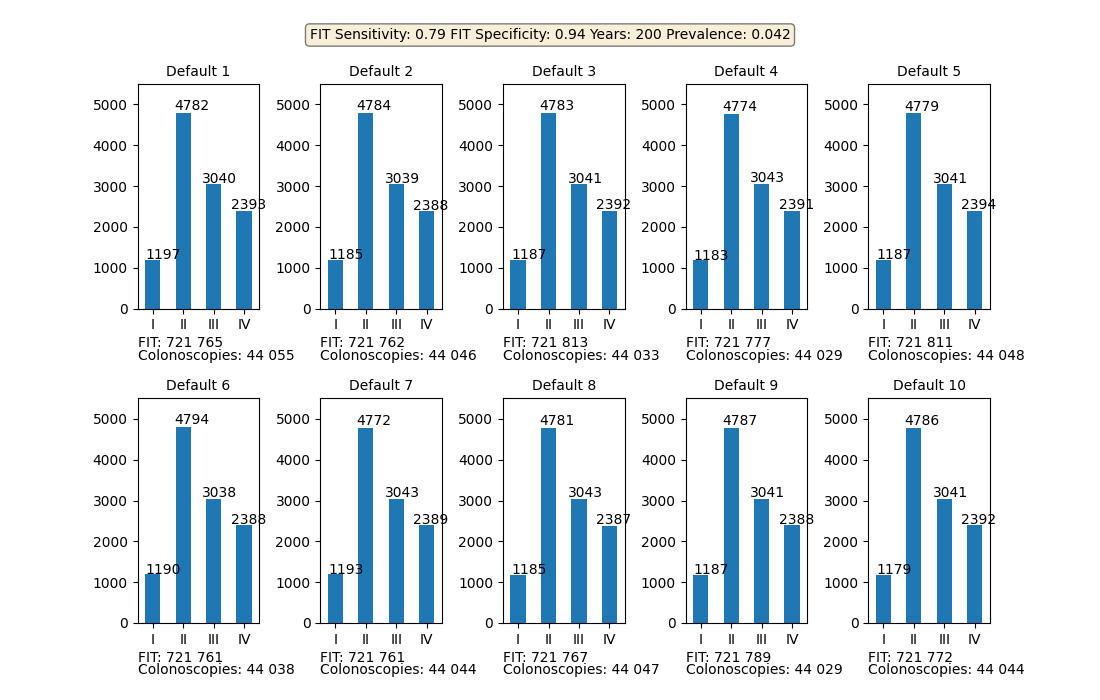
\includegraphics[width=1\textwidth]{images/5.results/treatments_for_defaults.png}
    \caption{Treatments for Default Replicas}
    \label{fig:treatments_for_default_replicas}
\end{figure}

Figure \ref{fig:treatments_for_default_replicas} illustrates that there are no notable changes in CRC stage distributions, and the number of FIT and colonoscopy procedures remains consistent across all scenarios.

\begin{figure}[H]
    \centering
    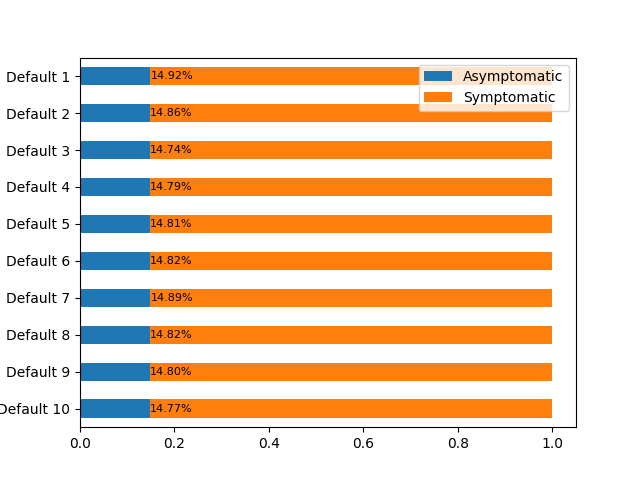
\includegraphics[width=1\textwidth]{images/5.results/screening_efficacy_for_defaults.png}
    \caption{Screening Efficacy for Default Replicas}
    \label{fig:screening_efficacy_for_default_replicas}
\end{figure}

In Figure \ref{fig:screening_efficacy_for_default_replicas}, the screening efficacy shows minor variations, with the most significant difference observed between scenarios amounting to a 0.18\% difference.

\begin{figure}[H]
    \centering
    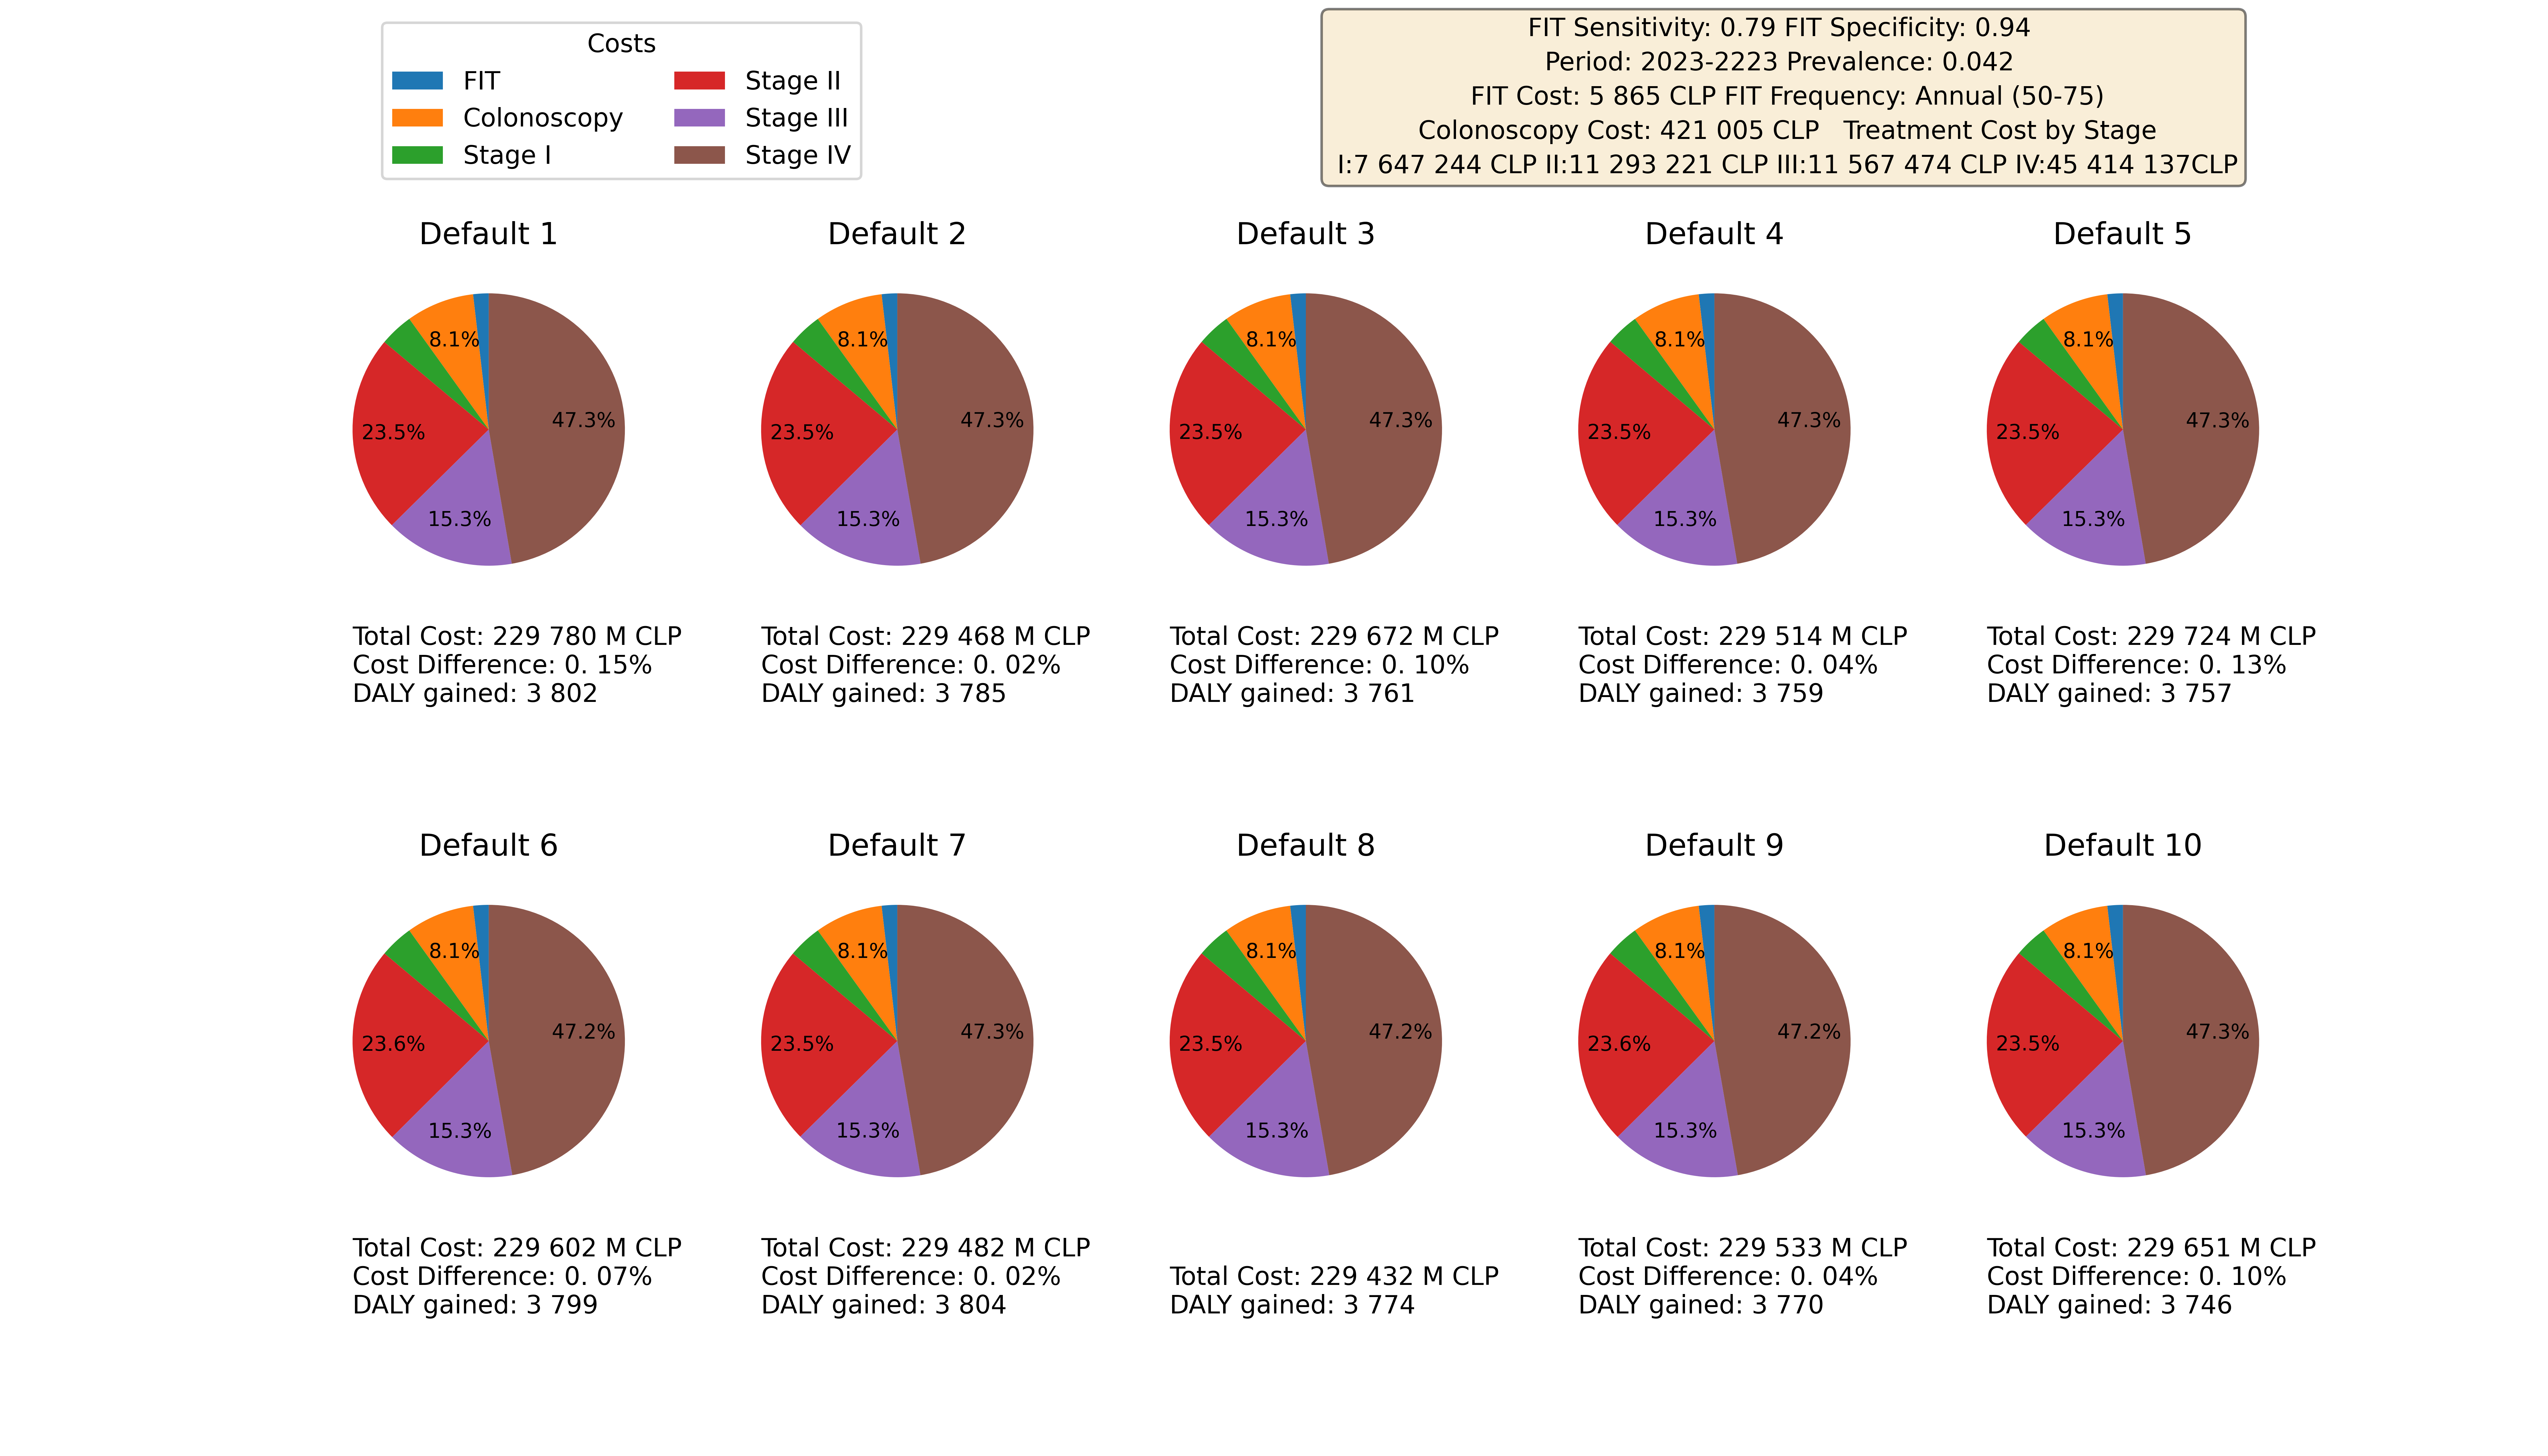
\includegraphics[width=1\textwidth]{images/5.results/costs_for_defaults.png}
    \caption{Costs for Default Replicas}
    \label{fig:costs_for_default_replicas}
\end{figure}

Figure \ref{fig:costs_for_default_replicas} depicts a consistent cost ratio across all scenarios. 'Default 8' is considered the baseline cost, being the lowest among all scenarios. The largest total cost difference between scenarios amounts to less than 0.2\%.

In conclusion, the replicas do not significantly impact this simulation model, as the variation between scenarios with the same parameters is negligible.

\section{Sensitivity Analysis: Screening Frequency}

In the simulation, we chose a biennial screening interval for FIT exams based on advice from a medical advisor. However, it's crucial to explore the effects of different screening frequencies to develop the best screening policy. This analysis aims to understand how the screening strategy's effectiveness is impacted by less or more frequent screenings. It's important to mention that these simulations spanned 200 years to reduce noise from the initial year and the adherence rate was set at 80\% for all scenarios.

\begin{figure}[H]
    \centering
    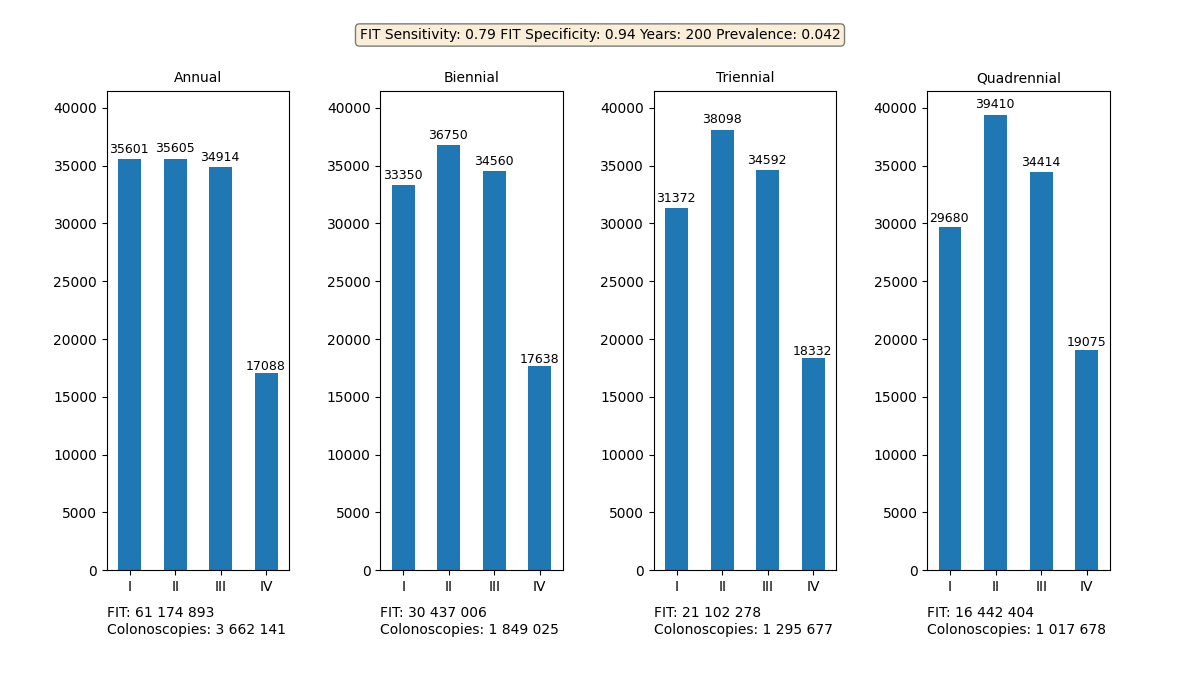
\includegraphics[width=1\textwidth]{images/5.results/treatments_by_frequency.png}
    \caption{Treatments by Screening Frequency}
    \label{fig:treatments_by_frequency}
\end{figure}

Figure \ref{fig:treatments_by_frequency} illustrates a significant decrease in the number of FIT and colonoscopy exams as the screening intervals increase. Moving from an annual to a biennial strategy notably reduces the number of exams conducted by half, and this reduction continues as the screening interval extends further to triennial and beyond.

\begin{figure}[H]
    \centering
    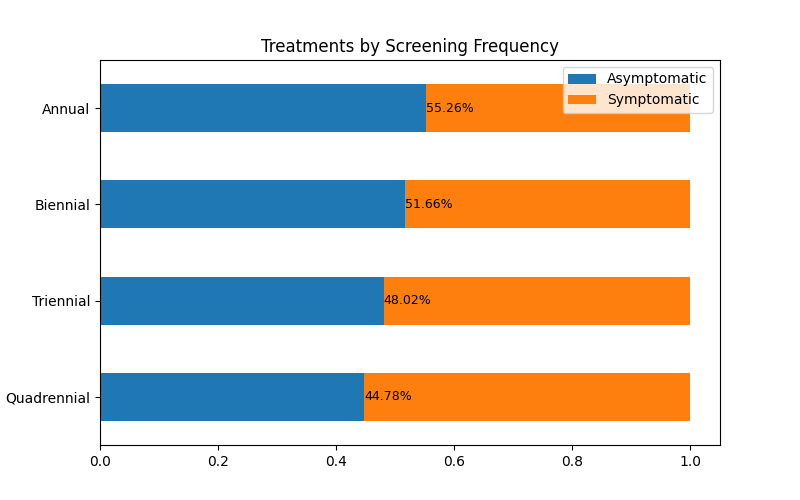
\includegraphics[width=1\textwidth]{images/5.results/screening_efficacy_by_frequency.png}
    \caption{Screening Efficacy by Frequency}
    \label{fig:screening_efficacy_by_frequency}
\end{figure}

Analyzing Figure \ref{fig:screening_efficacy_by_frequency}, transitioning from an annual to a biennial strategy reduces the number of exams, but there's a noticeable drop in performance of approximately 3\% each time the frequency is reduced.

\begin{figure}[H]
    \centering
    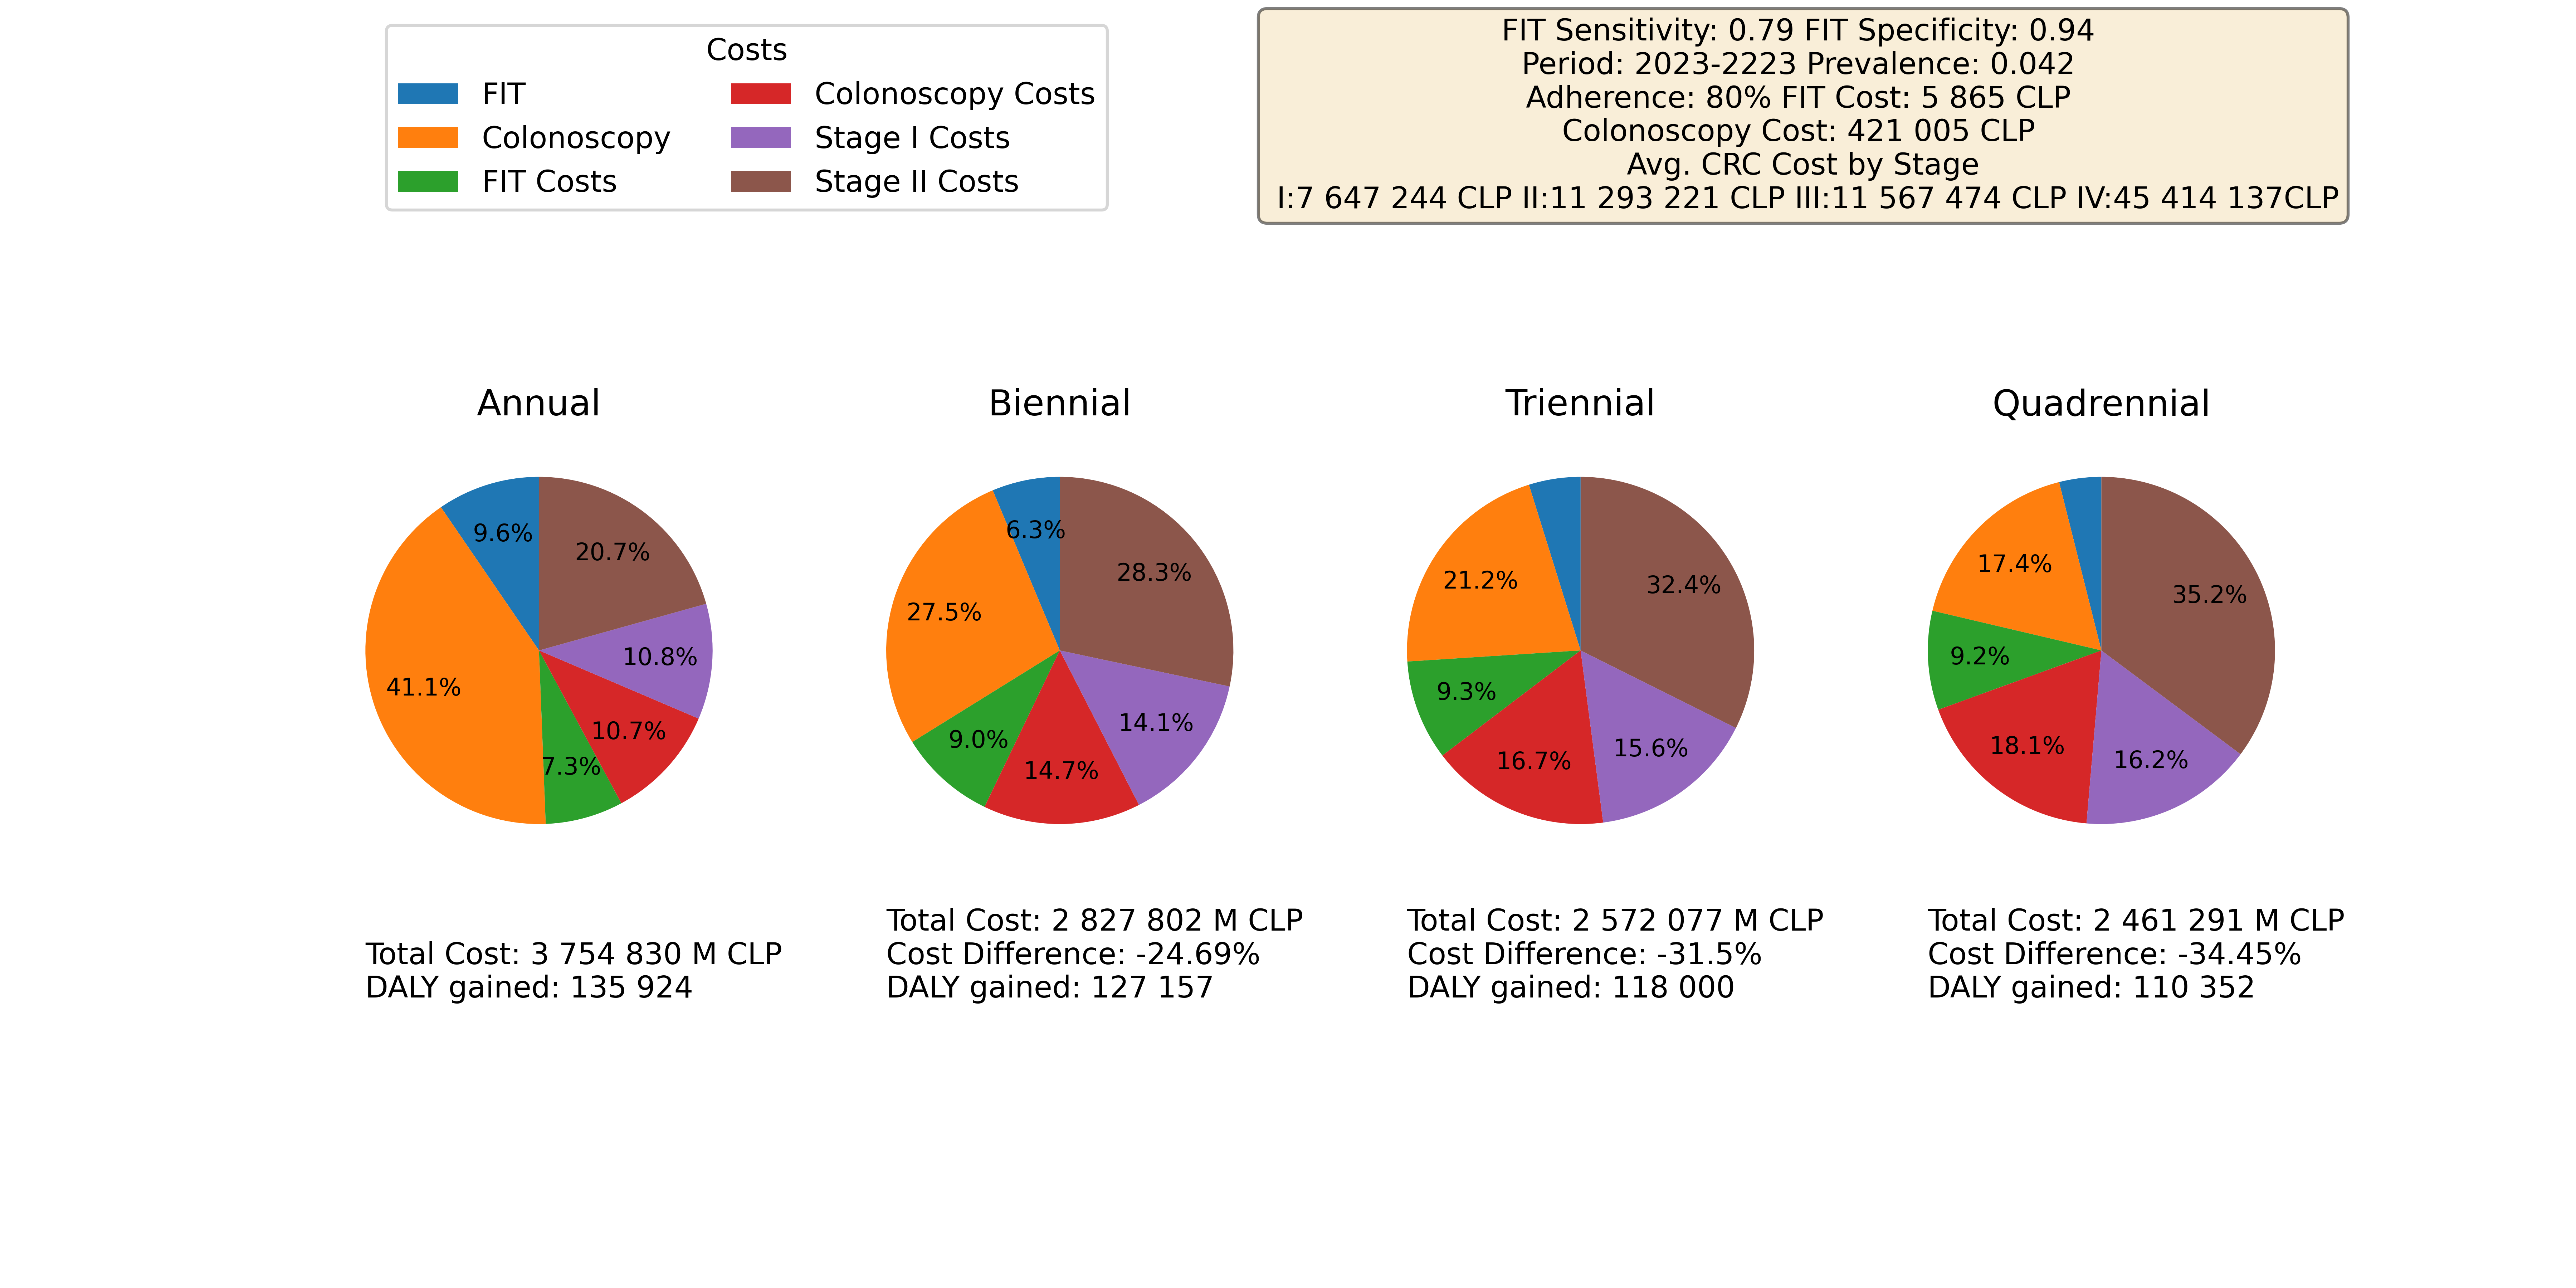
\includegraphics[width=1\textwidth]{images/5.results/costs_frequency.png}
    \caption{Costs by Frequency}
    \label{fig:costs_by_frequency}
\end{figure}

Now with Figure \ref{fig:costs_by_frequency} we can see that going from the annual strategy to the biennial strategy has a huge impact on the total costs of the system, reducing the costs by 25\%. Going from annual to triennial reduces the costs by 31\% so the reduction, even though it’s big, is not that significant.

In determining this parameter, an oncologist was consulted, providing insights into the optimal screening frequency. After reviewing the simulation's performances and associated costs, she concluded that while the cost reduction with a triennial screening was considerable, the corresponding performance metrics were not sufficiently robust. She cautioned against adopting a triennial screening interval, deeming it imprudent and advocating instead for a biennial screening strategy.

\section{Sensitivity Analysis: Screening Interval}

Currently, the screening interval spans from ages 50 to 75, encompassing a duration of 25 years for each individual. This timeframe aligns with the conventions observed in numerous European screening programs, which commonly adopt either this interval or the narrower range of 50 to 70 years. However, given the evolving landscape of life expectancy, alternative screening intervals warrant exploration to ascertain potentially superior outcomes. It's imperative to highlight that, to mitigate initial variability, the simulations were conducted over a 200-year span rather than the typical 20.

\begin{table}[H]
\caption{Simulations with different Screening Intervals}
\centering
\begin{tabular}{|c|c|c|c|}
\hline
Interval (years) & Total Cost M CLP & DALYs Gained & Efficacy Ratio\\ \hline
60-75 (15) & 2 600 602 (-8.4\%) & 82 086 (-35.4\%) & -4.21 \\ \hline
\rowcolor{lightred}
50-70 (20) & 2 748 535 (-3.2\%) & 113 373 (-10.8\%) & -3.39 \\ \hline
\rowcolor{lightred}
55-75 (20) & 2 735 710 (-3.7\%) & 107 962 (-15.1\%) & -4.13 \\ \hline
\textbf{50-75 (25)} & \textbf{2 839 398} & \textbf{127 150} &  \\ \hline
55-80 (25) & 2 826 202 (-0.5\%) & 116 735 (-8.2\%) & -17.62 \\ \hline
\rowcolor{lightgreen}
50-80 (30) & 2 976 125 (4.8\%) & 138 731 (9.1\%) & 1.89 \\ \hline
\rowcolor{lightgreen}
45-75 (30) & 2 996 982 (5.6\%) & 146 940 (15.5\%) & 2.8 \\ \hline
45-80 (35) & 3 082 601 (8.6\%) & 155 116 (22\%) & 2.57 \\ \hline
40-85 (45) & 3 362 547 (18.4\%) & 168 578 (32.6\%) & 1.77 \\ \hline
35-90 (55) & 3 595 708 (26.6\%) & 175 725 (38.2\%) & 1.43 \\ \hline
\end{tabular}
\subcaption*{The percentages are the differences between that simulation and the one with the \textbf{default parameters}. The Efficacy Ratio is the DALYs Gained Percentage divided by the Total Cost Percentage}
\label{table:simulation_intervals}
\end{table}

Table \ref{table:simulation_intervals} presents various options for selecting a new screening interval, each with its own cost and population impact considerations. Despite its apparent simplicity, this data provides valuable insights for budget adjustments.

For instance, if the goal is to expand the budget (highlighted in light green), lowering the starting age to 45 (45-75) yield better results in terms of DALYs gained per dollar spent than raising the upper age limit from 75 to 80 (50-80).

In contrast, if the aim is to reduce the budget (highlighted in light red), reducing the upper age limit from 75 to 70 (50-70) is more effective than increasing the starting age from 50 to 55 (55-75). While both approaches reduce the total costs, the 55 to 75 year interval produces a higher reduction in DALYs gained.

\section{Sensitivity Analysis: Colonoscopy Costs}

Conducting a sensitivity analysis on cost parameters is a standard practice in evaluating simulation models. This analysis allows us to understand how changes in cost parameters impact the feasibility of the proposed project. In Figure \ref{fig:costs_by_adherence}, we observe that at 80\% adherence, colonoscopy costs account for about 29\% of the total. However, the precise cost of a colonoscopy remains unclear due to significant variations in the obtained prices. Therefore, a sensitivity analysis on colonoscopy costs is called for.

The baseline parameter, which is the average cost across three clinics, provides a reference point for comparison. By individually assessing the influence of each clinic's cost on the simulation outcomes, we can examine how variations in this crucial parameter affect the overall results.

\begin{figure}[H]
    \centering
    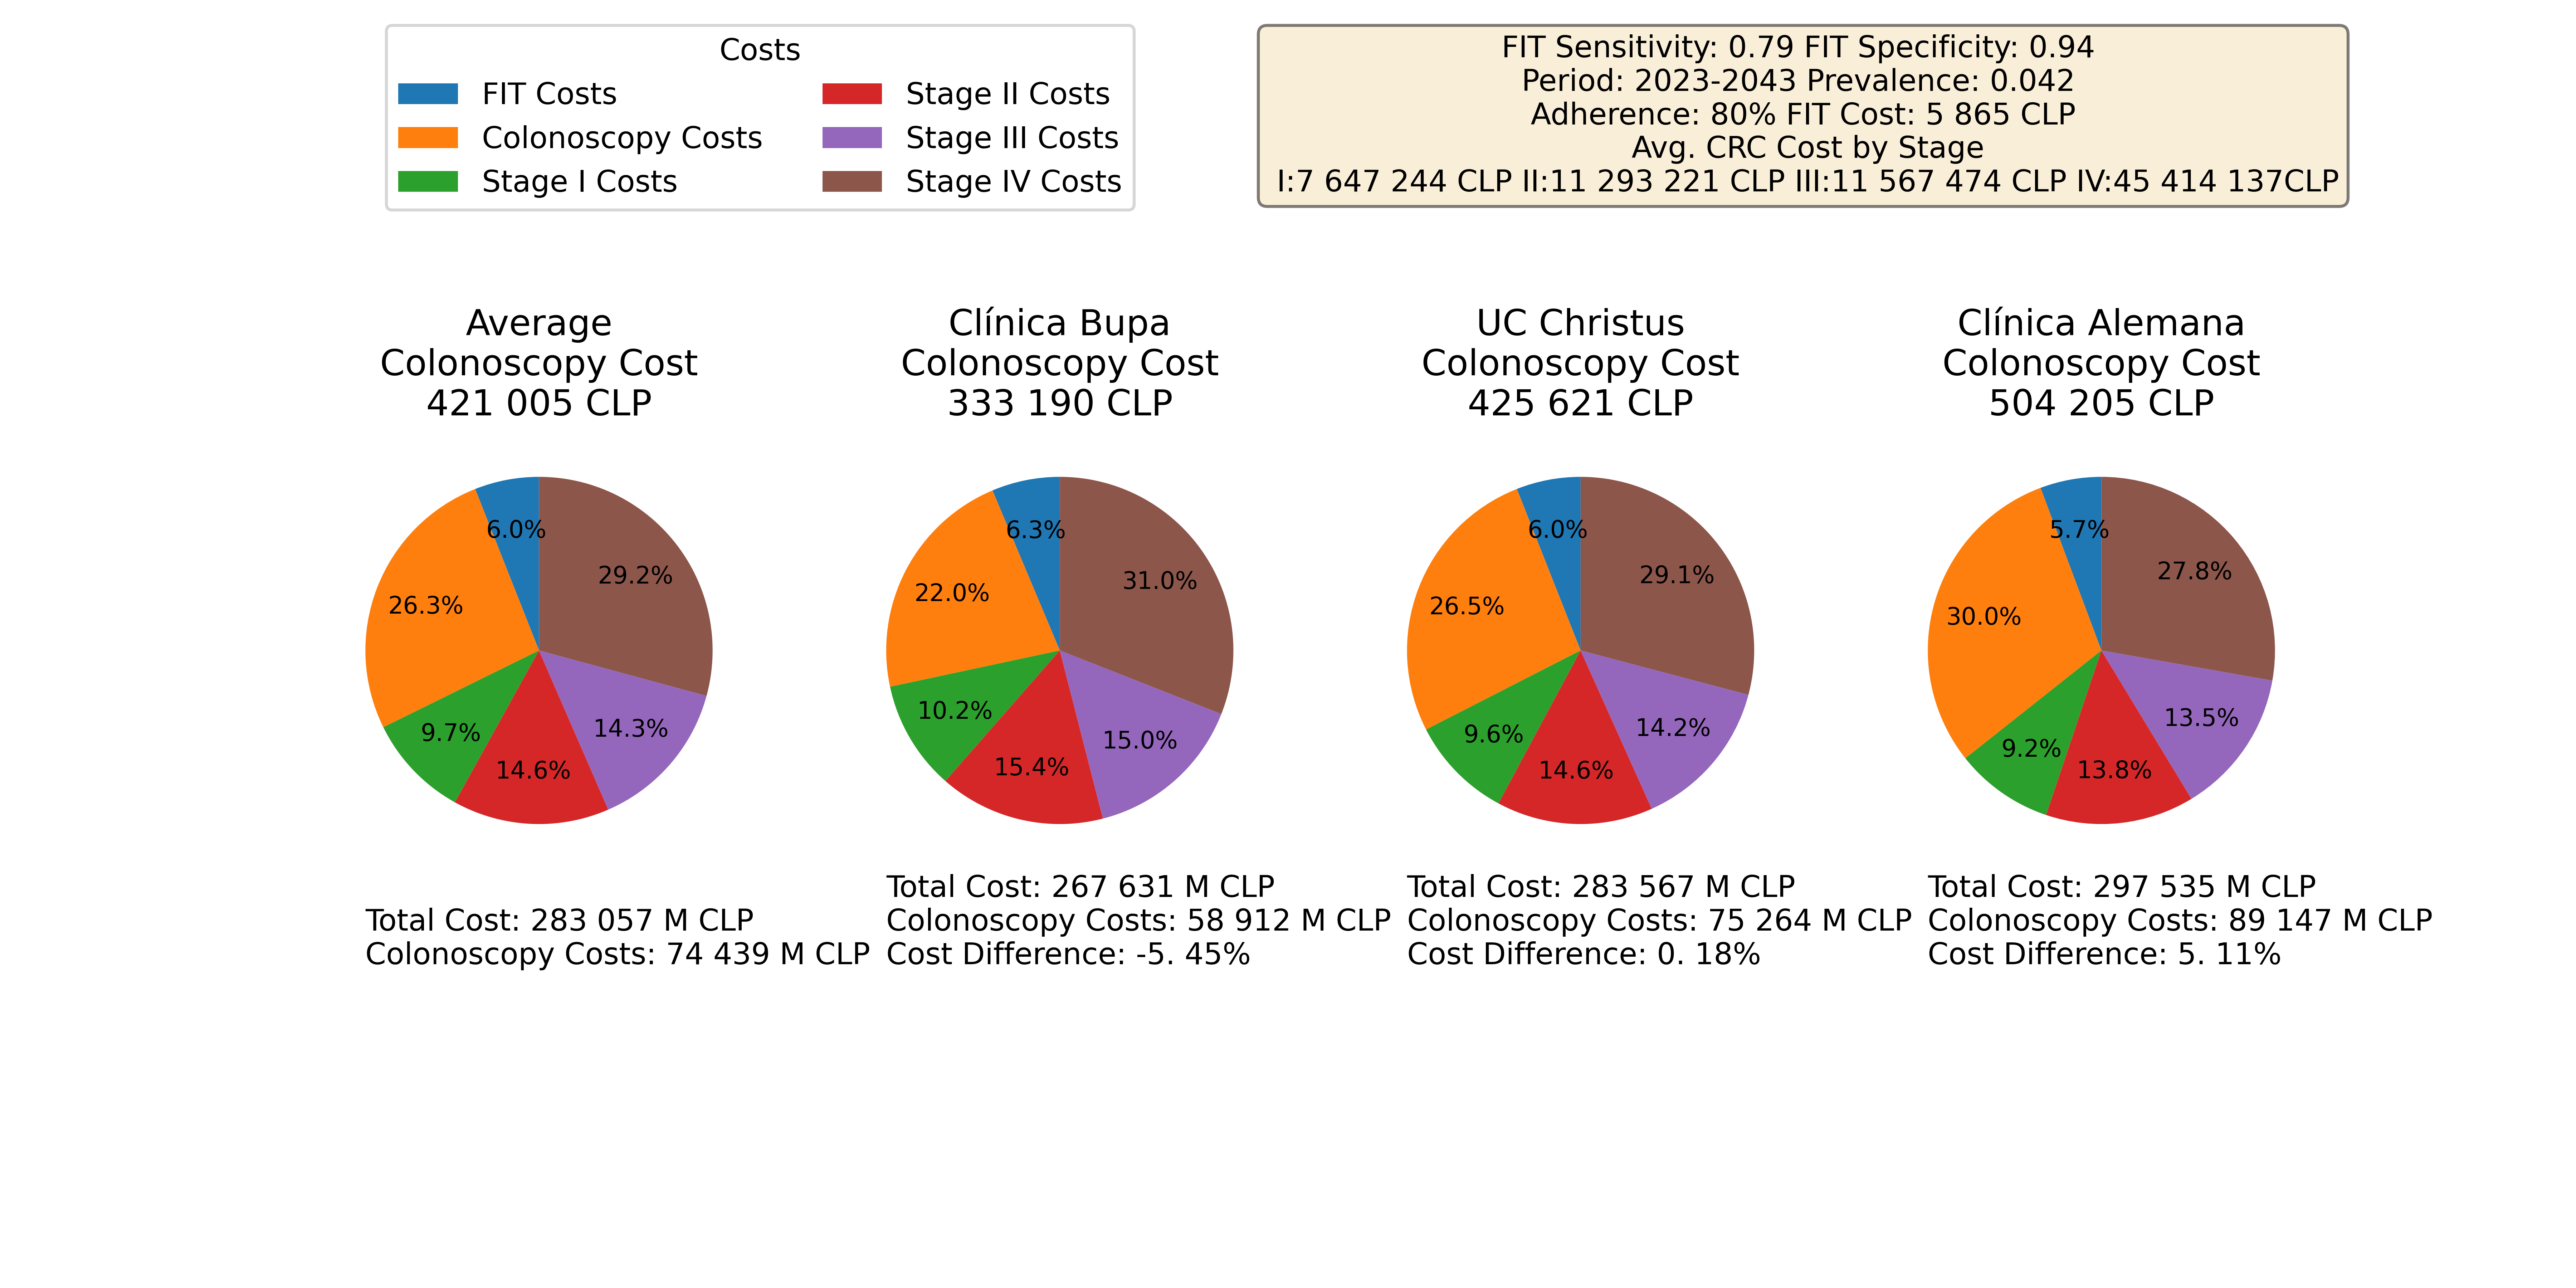
\includegraphics[width=1\textwidth]{images/5.results/costs_colonoscopies.png}
    \caption{Colonoscopy Costs}
    \label{fig:colonoscopy_costs}
\end{figure}

The charts in Figure \ref{fig:colonoscopy_costs} takes a look at how the colonoscopy exams affect the overall costs for screening colorectal cancer. It's clear that the cost of colonoscopy exams is an important part of managing the budget for colorectal cancer treatments as the lower and upper bound of total costs differentiate about 5\% from the average.

\section{Sensitivity Analysis: FIT Performance Indicators}

\subsection*{Improved Sensitivity}

The enhancement in sensitivity is expected to have a straightforward effect on the simulation. As the detection of patients with the disease improves or worsens, the percentage of asymptomatic detection should correspondingly improve or deteriorate. This adjustment is unlikely to significantly impact costs, as the main effect lies in potential shifts of treatments to earlier stages.

\begin{figure}[H]
    \centering
    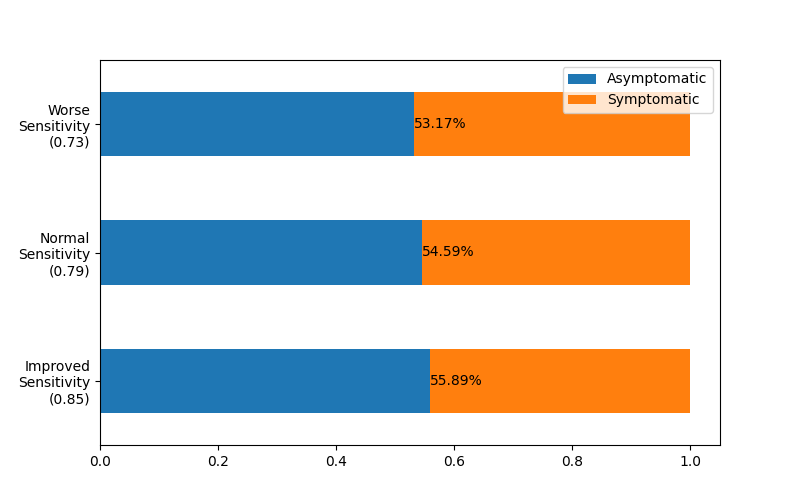
\includegraphics[width=1\textwidth]{images/5.results/screening_efficacy_by_fit_sensitivity.png}
    \caption{Screening Efficacy by FIT Sensitivity}
    \label{fig:screening_efficacy_by_sensitivity}
\end{figure}

In Figure \ref{fig:screening_efficacy_by_sensitivity} is observed that for every 6\% change in sensitivity, there's approximately a 1\% decrease or increase in asymptomatic detection. The impact on costs was minimal, representing around 0.1\% of the total cost.

\subsection*{Improved Specificity}

The improvement in specificity is expected to have a direct impact on the simulation costs. As the detection of patients without the disease improves or worsens, the number of false positives should accordingly decrease or increase. Since false positives require a colonoscopy, reducing their number results in an overall decrease in the cost of the entire system. Additionally, a scenario of almost perfect specificity was included to test the upper bound of this effect on the simulation.

\begin{figure}[H]
    \centering
    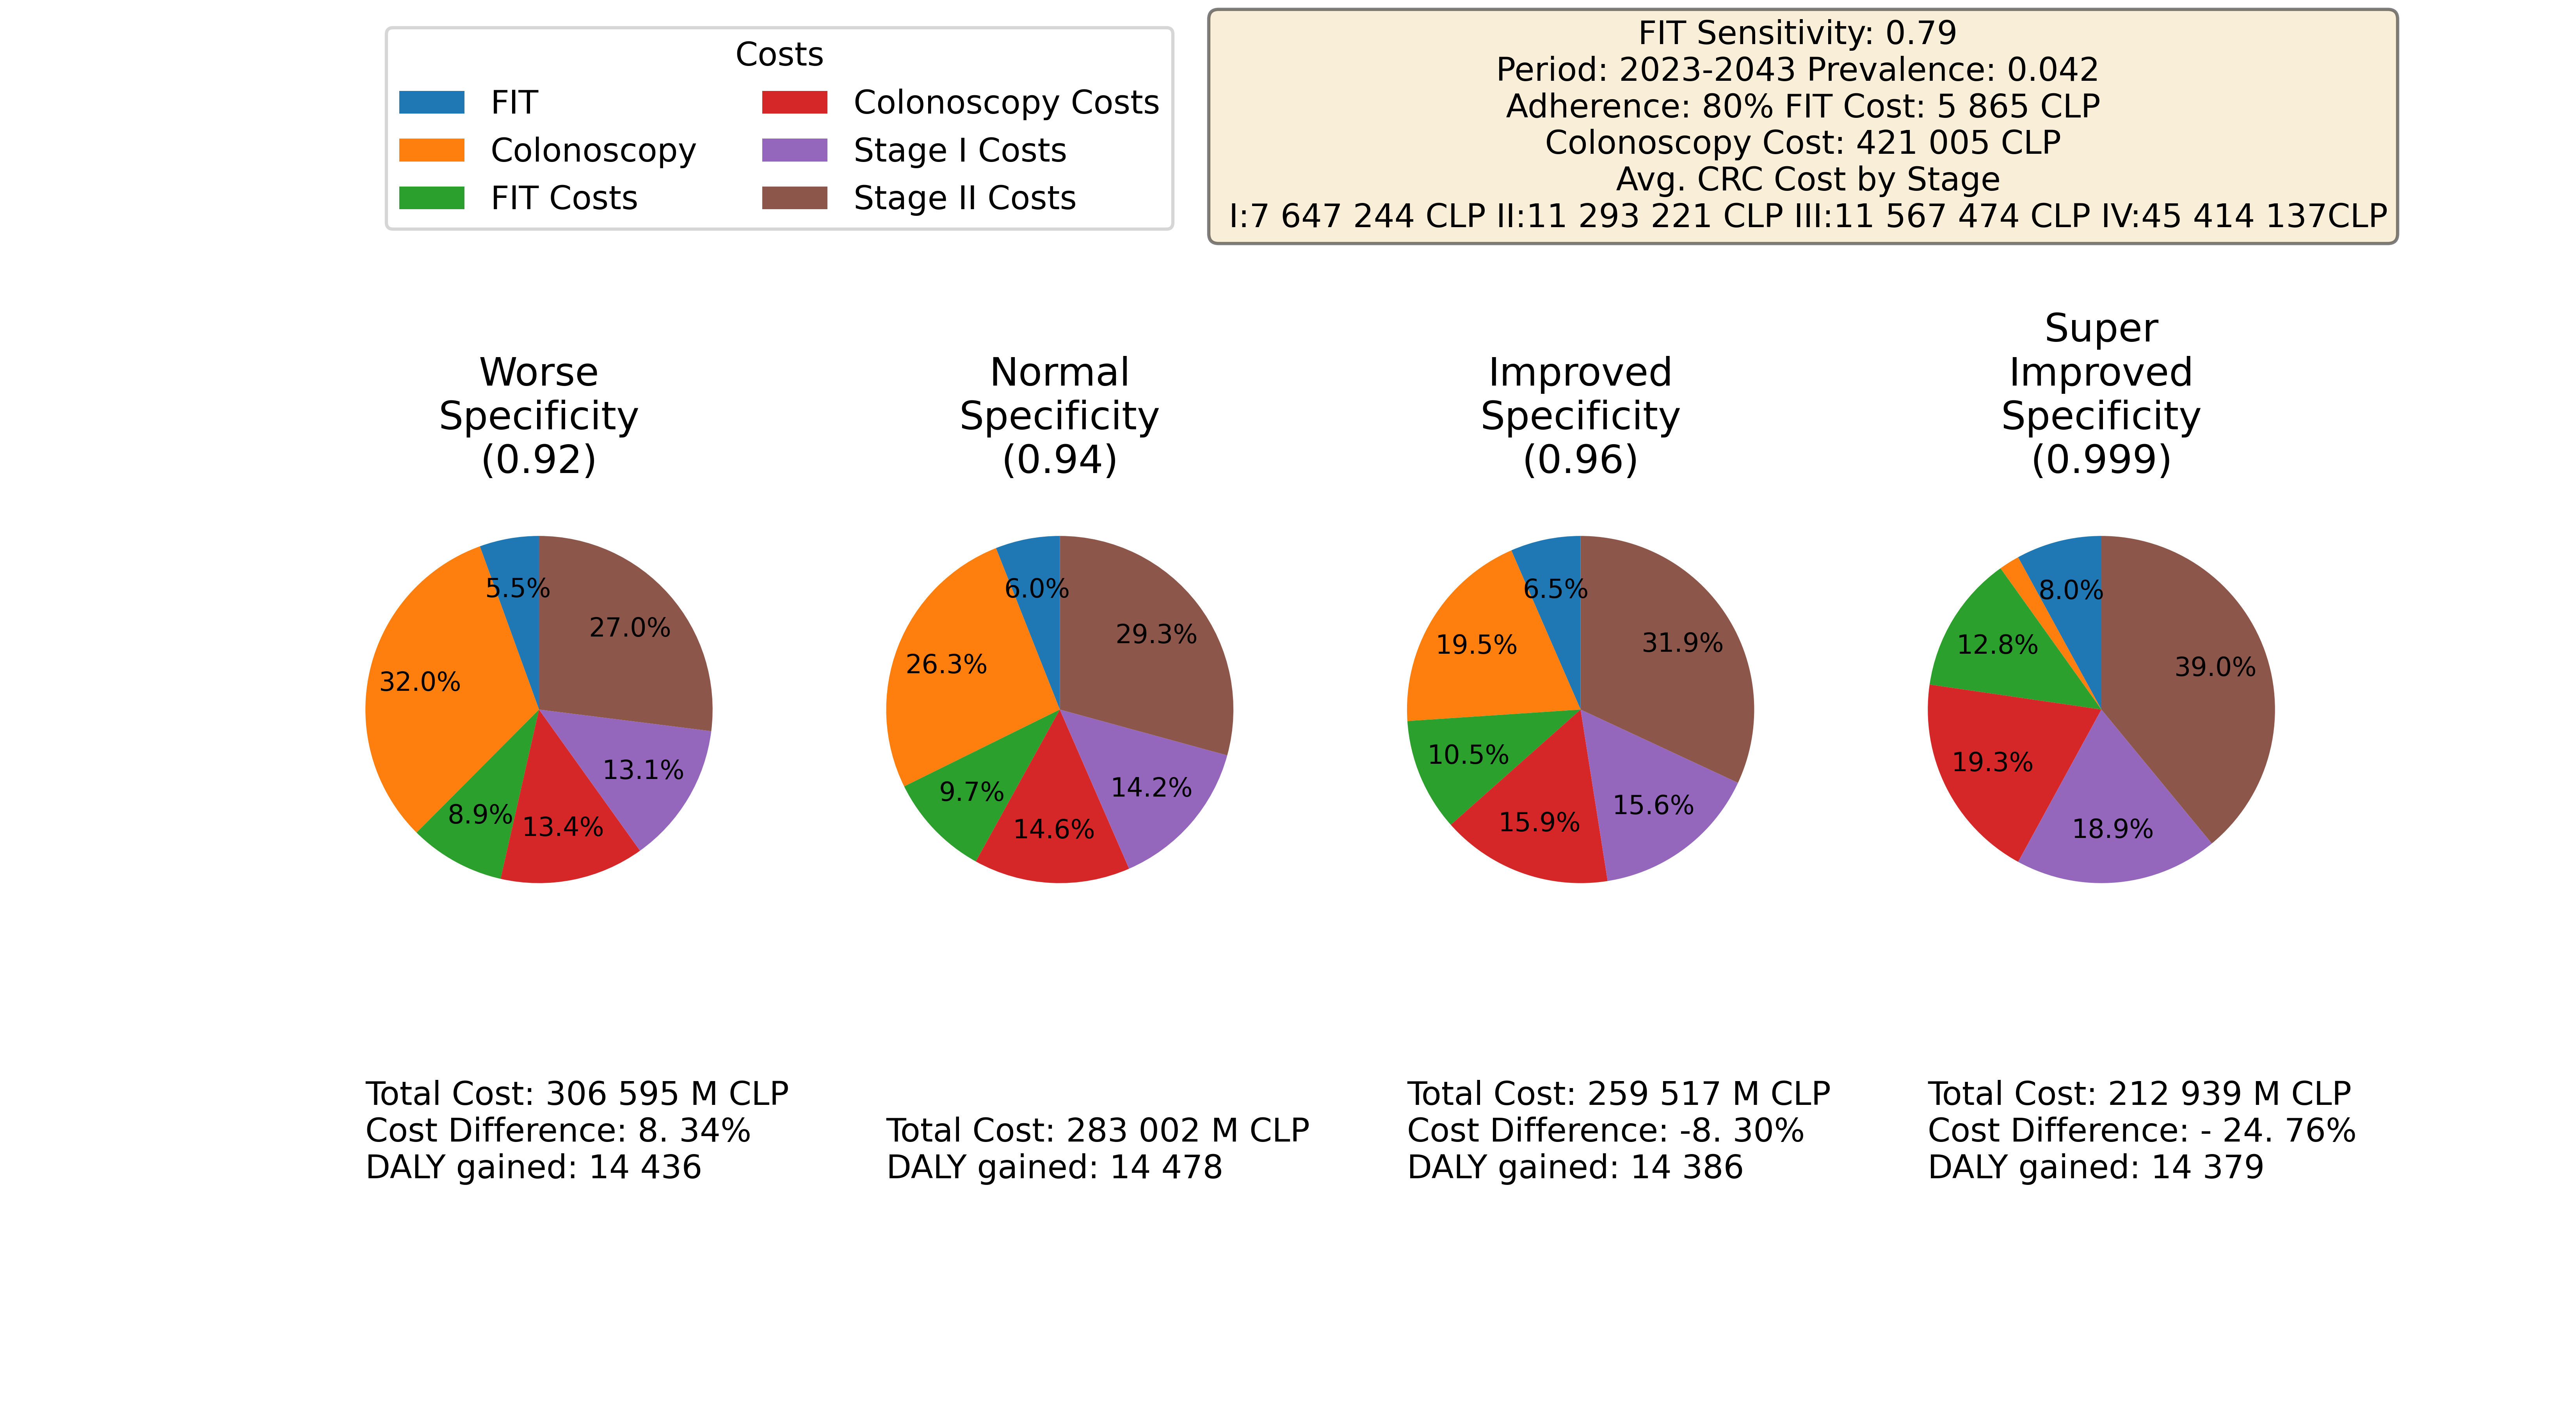
\includegraphics[width=1\textwidth]{images/5.results/costs_fit_specificity.png}
    \caption{Costs by FIT Specificity}
    \label{fig:costs_by_specificity}
\end{figure}

Figure \ref{fig:costs_by_specificity} illustrates the significant impact of improving or worsening the FIT specificity on the overall cost of the system. Even minor changes in specificity, such as a 2\% improvement or worsening, result in approximately a 8\% shift in the overall cost, highlighting its notable significance. When pushed to nearly perfect specificity, the screening strategy becomes cost-effective as the total cost is less than the 0\% adherence scenario in Figure \ref{fig:costs_by_adherence}.
